%%%%%%%%%%%%%%%%%%%%%%%%%%%%%%%%%%%%%%%%%
% Beamer Presentation
% LaTeX Template
% Version 1.0 (10/11/12)
%
% This template has been downloaded from:
% http://www.LaTeXTemplates.com
%
% License:
% CC BY-NC-SA 3.0 (http://creativecommons.org/licenses/by-nc-sa/3.0/)
%
%%%%%%%%%%%%%%%%%%%%%%%%%%%%%%%%%%%%%%%%%

%----------------------------------------------------------------------------------------
%	PACKAGES AND THEMES
%----------------------------------------------------------------------------------------

\documentclass[UTF8,aspectratio=169,14pt]{ctexbeamer}

\usepackage{hyperref}
\hypersetup{
	colorlinks=true,
	linkcolor=red,
	anchorcolor=blue,
	citecolor=green
}

\mode<presentation> {
	
	% The Beamer class comes with a number of default slide themes
	% which change the colors and layouts of slides. Below this is a list
	% of all the themes, uncomment each in turn to see what they look like.
	
	%\usetheme{default}
	%\usetheme{AnnArbor}
	%\usetheme{Antibes}
	%\usetheme{Bergen}
	%\usetheme{Berkeley}
	%\usetheme{Berlin}
	%\usetheme{Boadilla}
	%\usetheme{CambridgeUS}
	%\usetheme{Copenhagen}
	%\usetheme{Darmstadt}
	%\usetheme{Dresden}
	%\usetheme{Frankfurt}
	%\usetheme{Goettingen}
	%\usetheme{Hannover}
	%\usetheme{Ilmenau}
	%\usetheme{JuanLesPins}
	%\usetheme{Luebeck}
	\usetheme{Madrid}
	%\usetheme{Malmoe}
	%\usetheme{Marburg}
	%\usetheme{Montpellier}
	%\usetheme{PaloAlto}
	%\usetheme{Pittsburgh}
	%\usetheme{Rochester}
	%\usetheme{Singapore}
	%\usetheme{Szeged}
	%\usetheme{Warsaw}
	
	% As well as themes, the Beamer class has a number of color themes
	% for any slide theme. Uncomment each of these in turn to see how it
	% changes the colors of your current slide theme.
	
	%\usecolortheme{albatross}
	%\usecolortheme{beaver}
	%\usecolortheme{beetle}
	%\usecolortheme{crane}
	%\usecolortheme{dolphin}
	%\usecolortheme{dove}
	%\usecolortheme{fly}
	%\usecolortheme{lily}
	%\usecolortheme{orchid}
	%\usecolortheme{rose}
	%\usecolortheme{seagull}
	%\usecolortheme{seahorse}
	%\usecolortheme{whale}
	%\usecolortheme{wolverine}
	
	%\setbeamertemplate{footline} % To remove the footer line in all slides uncomment this line
	%\setbeamertemplate{footline}[page number] % To replace the footer line in all slides with a simple slide count uncomment this line
	
	%\setbeamertemplate{navigation symbols}{} % To remove the navigation symbols from the bottom of all slides uncomment this line
}

\usepackage{graphicx} % Allows including images
\graphicspath{{./figs/}}
\usepackage{booktabs} % Allows the use of \toprule, \midrule and \bottomrule in tables
\usepackage{longtable}
\usepackage{listings}
\usepackage{xcolor}
\lstset{numbers=left, %设置行号位置
	numberstyle=\tiny, %设置行号大小
	keywordstyle=\color{blue}, %设置关键字颜色
	commentstyle=\color[cmyk]{1,0,1,0}, %设置注释颜色
	frame=single, %设置边框格式
	escapeinside=``, %逃逸字符(1左面的键),用于显示中文
	%breaklines, %自动折行
	extendedchars=false, %解决代码跨页时,章节标题,页眉等汉字不显示的问题
	xleftmargin=2em,xrightmargin=2em, aboveskip=1em, %设置边距
	tabsize=4, %设置tab空格数
	showspaces=false %不显示空格
}
% Fonts
% \usepackage{libertine}
% \setmonofont{Courier}
\setCJKsansfont[ItalicFont=Noto Serif CJK SC Black, BoldFont=Noto Sans CJK SC Black]{Noto Sans CJK SC}


%----------------------------------------------------------------------------------------
%	TITLE PAGE
%----------------------------------------------------------------------------------------

\title[第12讲]{第十二讲 :多处理器调度} % The short title appears at the bottom of every slide, the full title is only on the title page
\subtitle{第5节:BFS调度算法}
\author{向勇、陈渝、李国良} % Your name
\institute[清华大学] % Your institution as it will appear on the bottom of every slide, may be shorthand to save space
{
	清华大学计算机系 \\ % Your institution for the title page
	\medskip
	\textit{xyong,yuchen,liguoliang@tsinghua.edu.cn} % Your email address
}
\date{\today} % Date, can be changed to a custom date


\begin{document}

\begin{frame}
\titlepage % Print the title page as the first slide
\end{frame}

%----------------------------------------------
\begin{frame}
\frametitle{提纲} % Table of contents slide, comment this block out to remove it
\tableofcontents % Throughout your presentation, if you choose to use \section{} and \subsection{} commands, these will automatically be printed on this slide as an overview of your presentation
\end{frame}
%----------------------------------------------
%%	PRESENTATION SLIDES
%----------------------------------------------
\section{第5节:BFS(Brain Fuck Scheduler)调度算法} % Sections can be created in order to organize your presentation into discrete blocks, all sections and subsections are automatically printed in the table of contents as an overview of the talk
%----------------------------------------------
\subsection{BFS工作原理} % A subsection can be created just before a set of slides with a common theme to further break down your presentation into chunks
%----------------------------------------------
\begin{frame}[fragile]
    \frametitle{BFS工作原理}
    \framesubtitle{出处:\href{http://vellvisher.github.io/papers_reports/doc/BFS_FreeBSD.pdf}{Analysis of the BFS Scheduler in FreeBSD}}
% http://vellvisher.github.io/papers_reports/doc/BFS_FreeBSD.pdf
% Analysis of the BFS Scheduler in FreeBSD
    BFS调度算法是一种时间片轮转算法的变种.
%% figure
    \begin{figure}
%    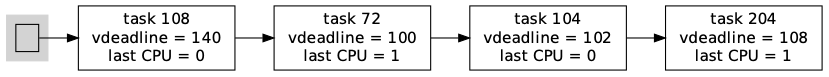
\includegraphics[width=1.0\linewidth]{figs/bfs-struct.png}
%    \caption{xxxx}
    \end{figure} \pause

在多处理机情况的单就绪队列(双向链表)选择,增加了队列互斥访问的开销,但减少了负载均衡算法开销。

\end{frame}
%----------------------------------------------
% #### BFS数据结构
% https://www.cs.unm.edu/~eschulte/classes/cs587/data/bfs-v-cfs_groves-knockel-schulte.pdf
% BFS vs.CFS Scheduler Comparison
% 
% P7: Figure4: BFS data structure
% 
% ![bfs-struct](figs/bfs-struct.png)
% 
% 在多处理机情况的单就绪队列(双向链表)选择,增加了队列互斥访问的开销,但减少了负载均衡算法开销。
% 
% #### BFS工作原理
% 
% http://vellvisher.github.io/papers_reports/doc/BFS_FreeBSD.pdf
% Analysis of the BFS Scheduler in FreeBSD
% 
% BFS调度算法是一种时间片轮转算法的变种。
% 
%----------------------------------------------
\begin{frame}[fragile]
    \frametitle{BFS就绪队列}
%    \subframetitle{yyyy}
%% block
    \begin{block}{线程优先级:有103个优先级}
	    \begin{itemize}
	        \item 100个静态的实时优先级;
	        \item 3个普通优先级SCHEDISO (isochronous)、SCHEDNORMAL和SCHEDIDLEPRIO (idle priority scheduling);
% BFS有103个优先级,其中100个静态的实时优先级,3个普通优级SCHEDISO (isochronous)、SCHEDNORMAL和SCHEDIDLEPRIO (idle priority scheduling);
	    \end{itemize}
    \end{block} \pause
%% block
    \begin{block}{单就绪队列}
	    \begin{itemize}
	        \item 所有CPU共享一个双向链表结构的单就绪队列;
	        \item 所有线程按优先级排队;
	        \item 相同优先级的每个线程有一个时间片长度和虚拟截止时间;
	    \end{itemize}
    \end{block}
\end{frame}
% ##### 单就绪队列
% 
% 1. 所有CPU共享一个双向链表结构的单就绪队列;
% 2. 所有线程按优先级排队;
% 3. 相同优先级的每个线程有一个时间片长度和虚拟最长等待时间;
% 

%----------------------------------------------
\begin{frame}[fragile]
%    \frametitle{虚拟截止时间(Virtual Deadline)}
%    \subframetitle{yyyy}
%% block
    \begin{block}{时间片大小}
    时间片大小由算法参数指定,可在1ms到1000ms间选择,缺省设置为6ms;
    \end{block} \pause

%% block
    \begin{block}{虚拟截止时间(Virtual Deadline)}
    \begin{itemize}
        \item 它是一个关于就绪队列中线程等待CPU最长时间的排序,并不是真实的截止时间; \pause
        \item 线程时间片用完时,重新计算虚拟截止时间;
        \item 事件等待结束时,虚拟截止时间保持不变,以抢先相同优先级的就绪线程; \pause
        \item 为了让线程在上次运行的CPU上运行,不同CPU对线程的虚拟截止时间加一个权重;
    \end{itemize}
    \end{block}

\end{frame}

% ##### 时间片大小选择
% 
% 由算法参数指定,可在1ms到1000ms间选择,缺省设置为6ms;
% 
% ##### 虚拟截止时间(Virtual Deadline)
% 
%  1. 它是一个关于就绪队列中线程等待CPU最长时间的排序,并不是真实的截止时间;
%  2. 为了让线程在上次运行的CPU上运行,不同CPU对线程的虚拟截止时间加一个权重;
%   3. 线程时间片用完时,重新计算虚拟截止时间;
%   4. 事件等待结束时,虚拟截止时间保持不变,以抢先相同优先级的就绪线程;
% 
% ##### 线程优先级
% 
% BFS有103个优先级,其中100个静态的实时优先级,3个普通优级SCHEDISO (isochronous)、SCHEDNORMAL和SCHEDIDLEPRIO (idle priority scheduling);
% 
%----------------------------------------------
\begin{frame}[fragile]
    \frametitle{虚拟截止时间计算}
%    \subframetitle{yyyy}

依据当前时间、线程优先级和时间片设置计算;

%% lstlisting
    \begin{lstlisting}[language = C]
offset = jiffies + (prior_atio ∗ rr_interval)
prioratio increases by 10% for every nice level
    \end{lstlisting}

\pause
虚拟截止时间计算结果: \href{https://wikimili.com/en/Brain_Fuck_Scheduler}{https://wikimili.com/en/Brain\_Fuck\_Scheduler}
\end{frame}
% ##### 虚拟截止时间计算
% 
% 依据当前时间、线程优先级和时间片设置计算;
% 
% offset = jiffies + (prior_atio ∗ rr_interval)
% prioratio increases by 10% for every nice level
% 
% 虚拟截止时间计算结果: https://wikimili.com/en/Brain_Fuck_Scheduler
%----------------------------------------------
\begin{frame}[fragile]
    \frametitle{相关线程状态置换}
 %   \subframetitle{yyyy}
    \begin{itemize}
        \item 时间片用完:重新设置虚拟截止时间后,插入就绪队列;
        \item 等待事件出现:虚拟截止时间保持不变,抢先低优先级线程或插入就绪队列;
    \end{itemize}

\end{frame}
% ##### 相关线程状态置换
% 
% 时间片用完:重新设置虚拟截止时间后,插入就绪队列;
% 
% 事件等待结束:虚拟截止时间保持不变,抢先低优先级线程或插入就绪队列;
% 
%----------------------------------------------
\subsection{BFS与CFS的性能对比} % A subsection can be created just before a set of slides with a common theme to further break down your presentation into chunks
%----------------------------------------------
\begin{frame}[fragile]
    \frametitle{BFS与CFS的性能对比(2012)}
    \framesubtitle{测试硬件环境}
%% figure
    \begin{figure}
    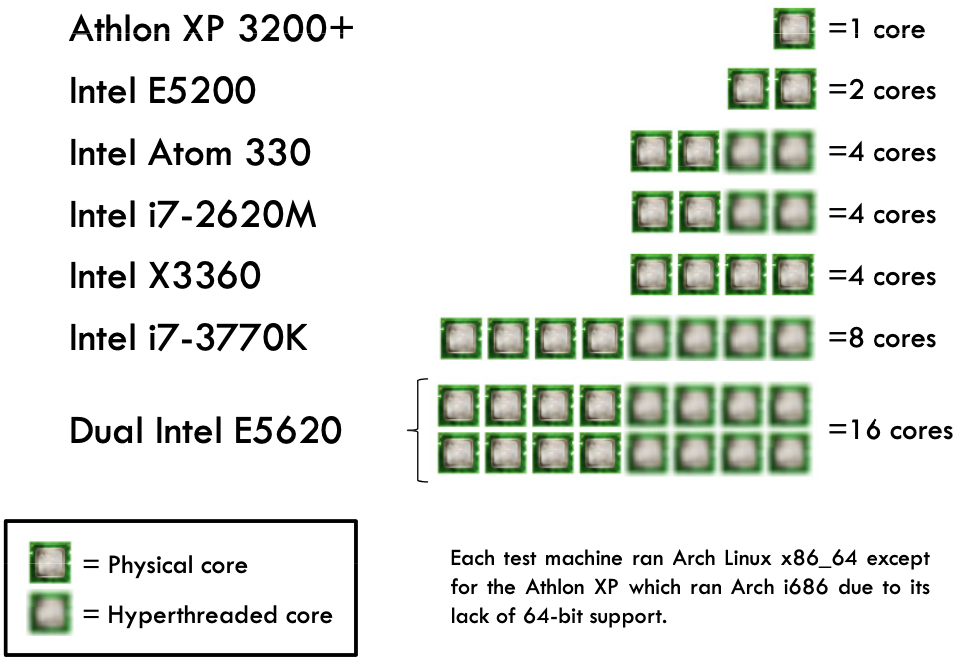
\includegraphics[width=0.6\linewidth]{test-machines}
%    \caption{xxxx}
    \end{figure}

\end{frame}
%----------------------------------------------
% ##### 测试硬件环境
% 
% ![test-machines](figs/test-machines.png)
% 
%----------------------------------------------
\begin{frame}[fragile]
    \frametitle{测试用例集}
%    \subframetitle{出处:\href{http://repo-ck.com/bench/cpu_schedulers_compared.pdf}{CPU Schedulers Compared}}
    \begin{itemize}
        \item Linux kernel v3.6.2.2的GCC编译
        \item Linux kernel v3.6.2内核源代码树的lrzip压缩
        \item 从720p到360p的MPEG2视频ffmpeg压缩
        \end{itemize}
\end{frame}
%----------------------------------------------
% #### BFS与CFS的性能对比(2012)
% http://repo-ck.com/bench/cpu_schedulers_compared.pdf
% CPU SCHEDULERS COMPARED
% 
% ##### 测试用例集
% 
% 1. Linux kernel v3.6.2.2的GCC编译
% 2. Linux kernel v3.6.2内核源代码树的lrzip压缩
% 3. 从720p到360p的MPEG2视频ffmpeg压缩
% 
%----------------------------------------------
\begin{frame}[fragile]
    \frametitle{压缩测试}
%    \subframetitle{yyyy}
%% figure
    \begin{figure}
    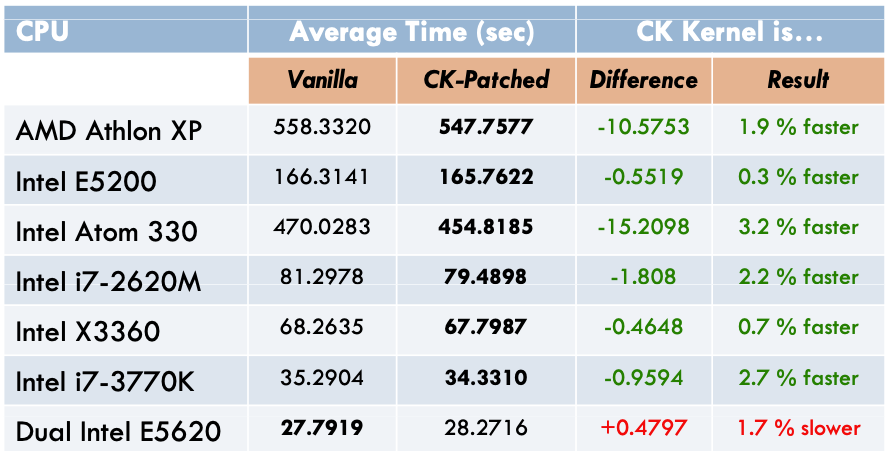
\includegraphics[width=0.8\linewidth]{compression-test}
%    \caption{xxxx}
    \end{figure}

\end{frame}
%----------------------------------------------
% ##### 压缩测试
% 
% ![compression-test](figs/compression-test.png)
% 
%----------------------------------------------
\begin{frame}[fragile]
    \frametitle{编译测试}
%    \subframetitle{yyyy}
%% figure
    \begin{figure}
    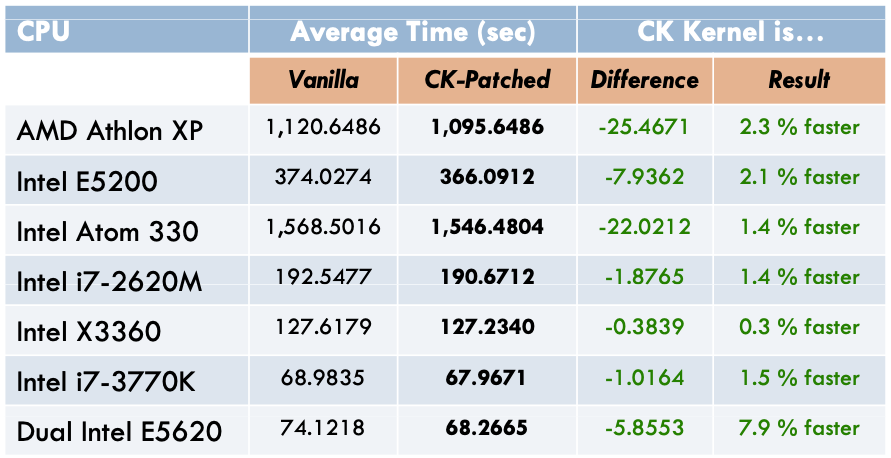
\includegraphics[width=0.8\linewidth]{make-test}
%    \caption{xxxx}
    \end{figure}

\end{frame}
%----------------------------------------------
% ##### 编译测试
% 
% ![make-test](figs/make-test.png)
% 
%----------------------------------------------
\begin{frame}[fragile]
    \frametitle{视频编码测试}
%    \subframetitle{yyyy}
%% figure
    \begin{figure}
    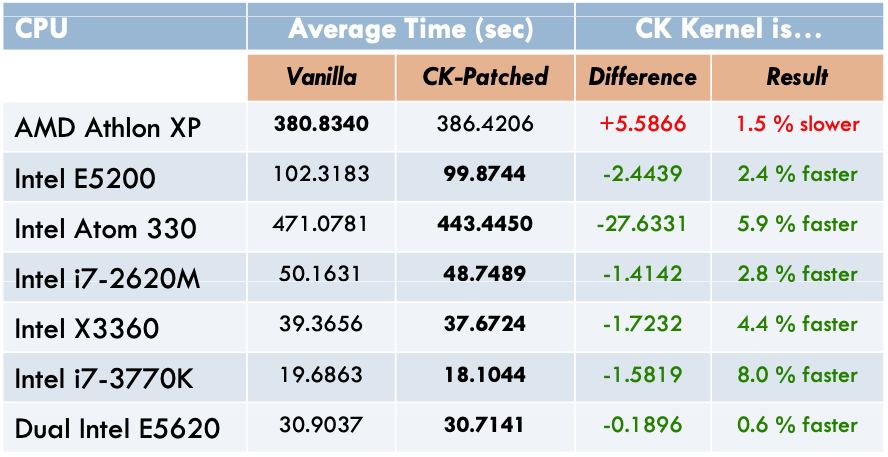
\includegraphics[width=0.8\linewidth]{video-test}
%    \caption{xxxx}
    \end{figure}

\end{frame}
% ##### 视频编码测试
% 
% ![video-test](figs/video-test.png)
%----------------------------------------------
\end{document}
